%%%%%%%%Bilecik �eyh Edebali �niversitesi M�hendsilik Fak�ltesi%%%%
%%%%%%%%%%%Bilgisayar M�hendisli�i Proje I-II �al��mas�%%%%%%%%%%%%
%%%%%%%%%%%%%%%%%%%%%%LaTeX Class%%%%%%%%%%%%%%%%%%%%%%%%%%%%%%%%%%
\documentclass{BUP}
%%%%%%%%%%%%%%%%%%%%%%%%%%%%%%%%%%%%%%%%%%%%%%%%%%%%%%%%%%%%%%%%%%%%%%%%%%%
\begin{document}
\shorthandoff{=}%grafik komutlar�nda babelden kaynaklanan hatay� engeller.
%%%%%%%%%%%%%Proje I-II �al��malar�n�n B�l�mleri%%%%%%%%%%%%%%%%%%%%%%%%%%%
\thispagestyle{empty} %Bu sayfaya sayfa numaralar� yaz�lmaz
\begin{figure}[H]
\centering
\includegraphics[scale=0.2]{logomuz}
%Bu komutla resim dosyam�z� y�kl�yoruz.
\end{figure}
%sa�a 4 sol 2 a�a�� yukar� 3%
\begin{center}
\textbf{T.C.}\\
\textbf{B�LEC�K �EYH EDEBAL� �N�VERS�TES�}\\
\textbf{M�HEND�SL�K FAK�LTES�}

\textbf{B�LG�SAYAR M�HEND�SL��� B�L�M�}
\end{center}

\vspace*{4cm}%bir miktar bo�luk b�rakmak i�in
\begin{center}
\textbf{Kartezyen �arp�m ve Kartezyen Yard�mc� �arp�m� Toplam Matlab'da �� Boyutlu �F'sinin G�sterimi}

\textbf{Ey�p Furkan ARIKAN}

\textbf{Bulan�k Mant�k}
\end{center}

\vspace*{\fill}
\begin{center}
\textbf{Bulan�k Mant�k DANI�MANI : Do�. Dr. Cihan KARAKUZU}

\textbf{B�LEC�K}\\ 
\textbf{\today}
\end{center}

%\include{2ickapak}
\pagenumbering{roman}%romen rakamlar� kullan�lmaya ba�lan�yor.
\setcounter{page}{2}% sayfa numaras�n� ii'den ba�lat�l�yor.
%\include{3ozetabstract}
%\include{4tesekkur}
%\include{5icindekiler}
%\include{6simgelistesi}
%\include{7sekillistesi}
%\include{8tablolistesi}
\pagenumbering{arabic}%Sayfa numaralamas�n� arap rakamlar�yla yapar.
\setcounter{page}{1}%sayfa numaras�n� 1'den ba�lat�r.
\section{G�R��}
	\textbf{Kartezyen �arp�m / Yard�mc� �arp�m Toplam}
	\textbf{(Cartesion Product/Co-product)}
	
	A ve B s�ras�yla X ve Y uzaylar�nda iki bulan�k k�me i�in; 
	
	A ve B'nin kartezyen �arp�m� (AXB) XxY uzay�nda tan�ml� bir bulan�k k�medir. Bu k�menin �F'si ;
	
	M� AXB(x,y) = min (M� A(x),M� B(y))-> T-norm = min �zelinde.
	
	A ve B'nin kartezyen yard�mc� �arp�m� (A+B) XxY uzay�nda tan�ml� bir bulan�k k�medir, �F'si;
	
	M� A+B(x,y) = max(M� A(x),M� B(y))-> S-norm; max �zelinde olarak tan�mlan�r.
	
\section{Materyal ve Metodlar}

\textbf{Kartezyen �arp�m (Cartesion Product) ve �� Boyutlu �F}

  \texttt{clc;} komutu komut penceresini temizler. \texttt{clc;} komut penceresinden t�m metni temizler ve net bir ekran olu�turur. \texttt{clc;}'yi �al��t�rd�ktan sonra, daha �nce g�r�nt�lenen metni g�rmek i�in komut penceresindeki kayd�rma �ubu�u kullan�lamaz. Bununla birlikte, komut ge�mi�indeki ifadeleri geri �a��rmak i�in komut penceresindeki yukar� ok tu�lar�n� kullanabiliriz.
  
  \texttt{clr;} veya \texttt{clear all;} komutu ayn�d�r. Sadece yaz�mlar� biraz farkl�d�r. \texttt{clear all;} �al��ma alan�n�z� ve komut pencerenizi temizler, b�ylece yeniden ba�layabiliriz. Bu, t�m rakamlar� kapat�r.

\texttt{clr;} matlab� "s�f�rlamak" i�in h�zl� bir yoldur. Konsol ekran�nda yaz�lan veya haf�zada kay�tl� kodlar� ve bilgileri temizler.

\texttt{x=[0,1,2,3,4,5];} komutuyla x dizisini elemanlar�yla tan�mlad�m.

\texttt{muAx=[0,0,1,0.5,0,0];} komutuyla muA(x) i�in muAx dizisini elemanlar�yla tan�mlad�m.

\texttt{a=10;b=11;c=12;d=13;e=14;f=15;}

\texttt{y=[a,b,c,d,e,f];} komutlar�yla �nce a,b,c,d,e ve f de�i�kenlerine de�erler atad�m. Bunu y dizisini elemanlar�yla olu�tururken kulland�m.

\texttt{muBy=[0,0,0,0.5,1,1];} komutuyla muB(y) i�in muBy dizisini elemanlar�yla tan�mlad�m.

\texttt{for ii=1:6}

    \texttt{for jj=1:6}
    
        \texttt{KARcrpm(ii,jj)=min(muAx(ii),muBy(jj));}
        
    \texttt{end}
    
\texttt{end}

Yukar�daki komutlarla \texttt{ii} de�i�kenini 1'den 6'ya kadar birer birer ve \texttt{jj} de�i�kenini 1'den 6'ya kadar birer birer art�rd�m ve daha �nceden tan�mlamad���m kartezyen �arp�m anlam�ndaki KARcrpm iki boyutlu dizisine muA(x) ve muB(y) dizilerinin minimumunu (en az�n�) aktard�m.


\texttt{for ii=1:6}

    \texttt{for jj=1:6}
    
        \texttt{fprintf('KARcrpm[\%i,\%i] => \%i\\(sla�)n',ii,jj,KARcrpm(ii,jj));}
        
    \texttt{end}
    
    \texttt{fprintf('\\(sla�)n');}
    
\texttt{end}

Yukar�daki komutlarla \texttt{ii} de�i�kenini 1'den 6'ya kadar birer birer ve \texttt{jj} de�i�kenini 1'den 6'ya kadar birer birer art�rd�m ve daha �nceden tan�mlamad���m ve minimum (en az) �F de�erlerini ald���m kartezyen �arp�m anlam�ndaki KARcrpm iki boyutlu dizisinin elemanlar�n� alt alta olacak �ekilde ve dizinin bir di�er sat�r�na ge�erken bir alt sat�ra daha ge�ecek �ekilde konsol ekran�na yazd�rd�m.

\texttt{mesh(KARcrpm)} komutuyla �eklin �zerinde bir a� varm�� gibi KARcrpm dizisini �izdirdim.

\texttt{xlabel('y');}

\texttt{ylabel('x');}

\texttt{zlabel('Kartezyen �arp�m');}

 Yukar�daki komutlarla x,y ve z eksenlerini g�sterdim. x ve y ekseni ters ��kt��� i�in onlar� ters g�sterdim.

\texttt{title('Kartezyen �arp�m Sonucu - 3 Boyutlu �F');} 
komutuyla �eklin etiketini yazd�rd�m.

\textbf{Kartezyen Yard�mc� �arp�m (Cartesion Co-product) Toplam ve �� Boyutlu �F}

\texttt{clc;} komutu komut penceresini temizler. \texttt{clc;} komut penceresinden t�m metni temizler ve net bir ekran olu�turur. \texttt{clc;}'yi �al��t�rd�ktan sonra, daha �nce g�r�nt�lenen metni g�rmek i�in komut penceresindeki kayd�rma �ubu�u kullan�lamaz. Bununla birlikte, komut ge�mi�indeki ifadeleri geri �a��rmak i�in komut penceresindeki yukar� ok tu�lar�n� kullanabiliriz.
  
  \texttt{clr;} veya \texttt{clear all;} komutu ayn�d�r. Sadece yaz�mlar� biraz farkl�d�r. \texttt{clear all;} �al��ma alan�n�z� ve komut pencerenizi temizler, b�ylece yeniden ba�layabiliriz. Bu, t�m rakamlar� kapat�r.

\texttt{clr;} matlab� "s�f�rlamak" i�in h�zl� bir yoldur. Konsol ekran�nda yaz�lan veya haf�zada kay�tl� kodlar� ve bilgileri temizler.

\texttt{x=[0,1,2,3,4,5];} komutuyla x dizisini elemanlar�yla tan�mlad�m.

\texttt{muAx=[0,0,1,0.5,0,0];} komutuyla muA(x) i�in muAx dizisini elemanlar�yla tan�mlad�m.

\texttt{a=10;b=11;c=12;d=13;e=14;f=15;}

\texttt{y=[a,b,c,d,e,f];} komutlar�yla �nce a,b,c,d,e ve f de�i�kenlerine de�erler atad�m. Bunu y dizisini elemanlar�yla olu�tururken kulland�m.

\texttt{muBy=[0,0,0,0.5,1,1];} komutuyla muB(y) i�in muBy dizisini elemanlar�yla tan�mlad�m.

\texttt{for ii=1:6}

    \texttt{for jj=1:6}
    
        \texttt{KARycrpm(ii,jj)=max(muAx(ii),muBy(jj));}
        
    \texttt{end}
    
\texttt{end}

Yukar�daki komutlarla \texttt{ii} de�i�kenini 1'den 6'ya kadar birer birer ve \texttt{jj} de�i�kenini 1'den 6'ya kadar birer birer art�rd�m ve daha �nceden tan�mlamad���m kartezyen yard�mc� �arp�m anlam�ndaki KARycrpm iki boyutlu dizisine muA(x) ve muB(y) dizilerinin maximumunu (en fazlas�n�) aktard�m.


\texttt{for ii=1:6}

    \texttt{for jj=1:6}
    
        \texttt{fprintf('KARycrpm[\%i,\%i] => \%i\\(sla�)n',ii,jj,KARycrpm(ii,jj));}
        
    \texttt{end}
    
    \texttt{fprintf('\\(sla�)n');}
    
\texttt{end}

Yukar�daki komutlarla \texttt{ii} de�i�kenini 1'den 6'ya kadar birer birer ve \texttt{jj} de�i�kenini 1'den 6'ya kadar birer birer art�rd�m ve daha �nceden tan�mlamad���m ve maximum (en fazla) �F de�erlerini ald���m kartezyen yard�mc� �arp�m anlam�ndaki KARycrpm iki boyutlu dizisinin elemanlar�n� alt alta olacak �ekilde ve dizinin bir di�er sat�r�na ge�erken bir alt sat�ra daha ge�ecek �ekilde konsol ekran�na yazd�rd�m.

\texttt{mesh(KARcrpm)} komutuyla �eklin �zerinde bir a� varm�� gibi KARycrpm dizisini �izdirdim.

\texttt{xlabel('y');}

\texttt{ylabel('x');}

\texttt{zlabel('Kartezyen Yard�mc� �arp�m');}

 Yukar�daki komutlarla x,y ve z eksenlerini g�sterdim. x ve y ekseni ters ��kt��� i�in onlar� ters g�sterdim.

\texttt{title('Kartezyen Yard�mc� �arp�m Sonucu - 3 Boyutlu �F');} 
komutuyla �eklin etiketini yazd�rd�m.
%\include{11bolum2}
\section{SONU�LAR VE �NER�LER}
\textbf{Kartezyen �arp�m (Cartesion Product) ve �� Boyutlu �F}

�ekil a�a��dad�r.

\begin{figure}[H]
\centering
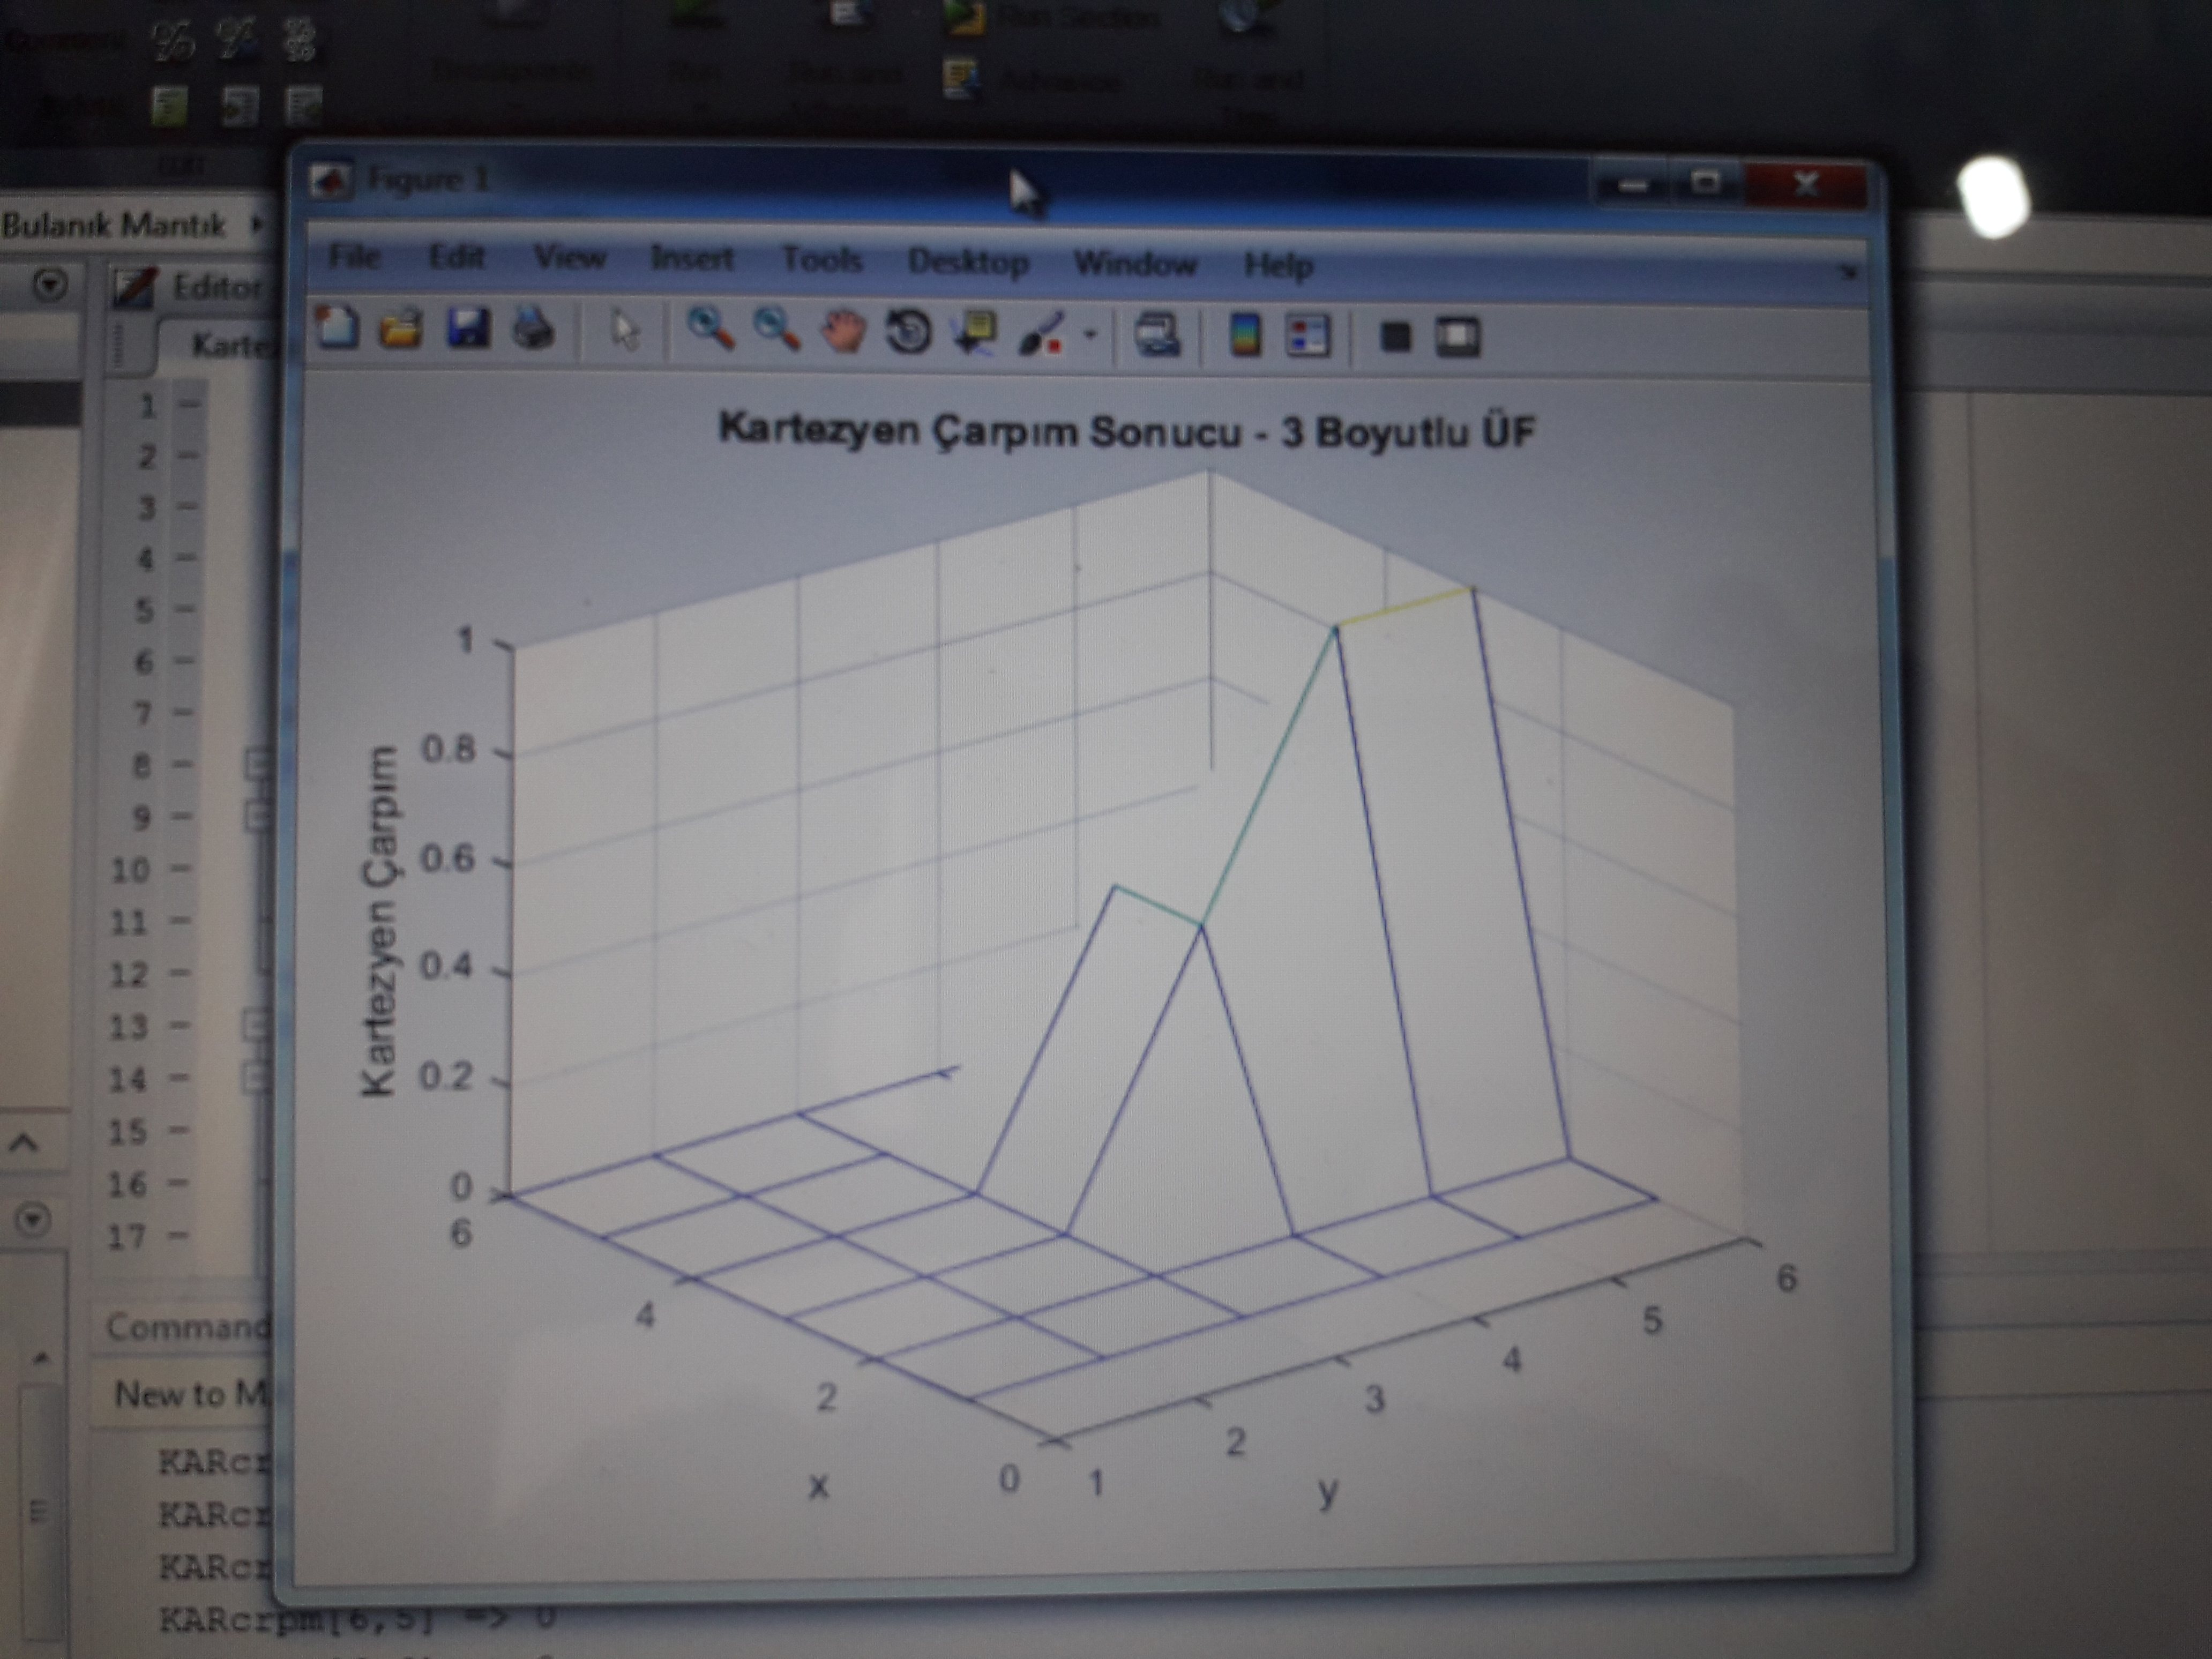
\includegraphics[scale=0.1]{Kartezyen_Carpim}
\caption{Kartezyen �arp�m (Cartesion Product) ve �� Boyutlu �F}
\end{figure}

x 2'ye giderken y d=13'te iken kartezyen �arp�m 0.5'tir.

x 2'ye giderken y e=14'te iken kartezyen �arp�m 1'dir.

x 2'ye giderken y f=15'te iken kartezyen �arp�m 1'dir.


x 3'e giderken y d=13'te iken kartezyen �arp�m 0.5'tir.

x 3'e giderken y e=14'te iken kartezyen �arp�m 0.5'tir.

x 3'e giderken y f=15'te iken kartezyen �arp�m 0.5'tir.

Di�er durumlarda kartezyen �arp�m s�f�rd�r.

\textbf{Kartezyen Yard�mc� �arp�m (Cartesion Co-product) Toplam ve �� Boyutlu �F}

�ekil a�a��dad�r.

\begin{figure}[H]
\centering
\includegraphics[scale=0.1]{Kartezyen_Yardimci_Carpim}
\caption{Kartezyen Yard�mc� �arp�m (Cartesion Co-product) Toplam ve �� Boyutlu �F}
\end{figure}

x 0'a giderken y d=13'te iken kartezyen yard�mc� �arp�m toplam 0.5'tir.

x 0'a giderken y e=14'te iken kartezyen yard�mc� �arp�m toplam 1'dir.

x 0'a giderken y f=15'te iken kartezyen yard�mc� �arp�m toplam 1'dir.


x 1'e giderken y d=13'te iken kartezyen yard�mc� �arp�m toplam 0.5'tir.

x 1'e giderken y e=14'te iken kartezyen yard�mc� �arp�m toplam 1'dir.

x 1'e giderken y f=15'te iken kartezyen yard�mc� �arp�m toplam 1'dir.


x 2'ye giderken y a=10'da iken kartezyen yard�mc� �arp�m toplam 1'dir.

x 2'ye giderken y b=11'de iken kartezyen yard�mc� �arp�m toplam 1'dir.

x 2'ye giderken y c=12'de iken kartezyen yard�mc� �arp�m toplam 1'dir.

x 2'ye giderken y d=13'te iken kartezyen yard�mc� �arp�m toplam 1'dir.

x 2'ye giderken y e=14'te iken kartezyen yard�mc� �arp�m toplam 1'dir.

x 2'ye giderken y f=15'te iken kartezyen yard�mc� �arp�m toplam 1'dir.


x 3'e giderken y a=10'da iken kartezyen yard�mc� �arp�m toplam 0.5'tir.

x 3'e giderken y b=11'de iken kartezyen yard�mc� �arp�m toplam 0.5'tir.

x 3'e giderken y c=12'de iken kartezyen yard�mc� �arp�m toplam 0.5'tir.

x 3'e giderken y d=13'te iken kartezyen yard�mc� �arp�m toplam 0.5'tir.

x 3'e giderken y e=14'te iken kartezyen yard�mc� �arp�m toplam 1'dir.

x 3'e giderken y f=15'te iken kartezyen yard�mc� �arp�m toplam 1'dir.


x 4'e giderken y d=13'te iken kartezyen yard�mc� �arp�m toplam 0.5'tir.

x 4'e giderken y e=14'te iken kartezyen yard�mc� �arp�m toplam 1'dir.

x 4'e giderken y f=15'te iken kartezyen yard�mc� �arp�m toplam 1'dir.


x 5'e giderken y d=13'te iken kartezyen yard�mc� �arp�m toplam 0.5'tir.

x 5'e giderken y e=14'te iken kartezyen yard�mc� �arp�m toplam 1'dir.

x 5'e giderken y f=15'te iken kartezyen yard�mc� �arp�m toplam 1'dir.


Di�er durumlarda kartezyen yard�mc� �arp�m toplam s�f�rd�r.

Not: Matlab dosyas�nda program kodlar�n� yazarken konsol ekran� ��kt�lar�n� da verdim.
\section{EKLER}

\textbf{Kartezyen Carpim (Cartesion Product)ve Uc Boyutlu UF}

\begin{verbatim}
clc;
clear all;
x=[0,1,2,3,4,5];
muAx=[0,0,1,0.5,0,0];
a=10;b=11;c=12;d=13;e=14;f=15;
y=[a,b,c,d,e,f];
muBy=[0,0,0,0.5,1,1];
for ii=1:6
    for jj=1:6
        KARcrpm(ii,jj)=min(muAx(ii),muBy(jj));
    end
end
for ii=1:6
    for jj=1:6
        fprintf('KARcrpm[%i,%i] => %i\n',ii,jj,KARcrpm(ii,jj));
    end
    fprintf('\n');
end
mesh(KARcrpm)
xlabel('y');
ylabel('x');
zlabel('Kartezyen Carpim');
title('Kartezyen Carpim Sonucu - 3 Boyutlu UF');
\end{verbatim}

\textbf{Kartezyen Yardimci Carpim (Cartesion Co-product) Toplam ve Uc Boyutlu UF}

\begin{verbatim}
clc;
clear all;
x=[0,1,2,3,4,5];
muAx=[0,0,1,0.5,0,0];
a=10;b=11;c=12;d=13;e=14;f=15;
y=[a,b,c,d,e,f];
muBy=[0,0,0,0.5,1,1];
for ii=1:6
    for jj=1:6
        KARycrpm(ii,jj)=max(muAx(ii),muBy(jj));
    end
end
for ii=1:6
    for jj=1:6
        fprintf('KARycrpm[%i,%i] => %i\n',ii,jj,KARycrpm(ii,jj));
    end
    fprintf('\n');
end
mesh(KARycrpm)
xlabel('y');
ylabel('x');
zlabel('Kartezyen Yardimci Carpim Toplam');
title('Kartezyen Yardimci Carpim Toplam Sonucu - 3 Boyutlu UF');
\end{verbatim}
\renewcommand{\refname}{KAYNAKLAR}
\addcontentsline{toc}{section}{KAYNAKLAR}
\begin{thebibliography}{99}%kaynak ortam� olu�turmak i�in
%%%%Kaynak We
\textcolor{red}{---> Kaynak yazar� bilinmeyen ulusal bir �al��madan al�nm�� ise:} Okuldaki lisans BM405 Bulan�k Mant�k ders notuna bakarak yap�lm��t�r.
\end{thebibliography}
%\include{15ozgecmis}
\shorthandon{=}
\end{document}
%%%%%%%%%%%%%%%%%%%%%%%%%%%B�TT�%%%%%%%%%%%%%%%%%%%%%%%%%%%%%%%%%%%%%%%%%%%%%